\section{Optical phonons in polar crystals}\label{sec:11.2}

A dark-matter particle of \SI{100}{keV} that scatters in GaAs through a light dark photon most often leaves behind one longitudinal optical phonon of \SI{36.35}{meV}. The dark photon does not couple to the nucleons. It couples to the charge, and when the gallium and arsenic sublattices move against each other every cell carries the dipole of their Born charges (\cref{sec:5.5}), whose field the electrons screen. In the acoustic waves of \cref{sec:11.1} the cell moves as a whole and stays neutral, and at long wavelength a coupling to charge has no vertex there; in the optical branch of GaAs its vertex is $Z^*/\varepsilon_\infty = 0.19$ per cell at every small momentum transfer (\cref{we:8-nucleon}). Silicon and germanium, whose Born charges vanish, have no such channel. A polar target enters the rate through one band integral of its loss function, and the crystals with the largest band integrals have the highest kinematic edges.

\subsection{The phonon loss function}\label{sec:11.2-loss}

A dark photon, heavy or light, couples to the charge-number density $n_Z$, and so does any particle with a small electric charge (\cref{we:8-darkphoton}). For this row \cref{sec:8.4} gave an exact answer: $S_{ZZ} = (2q^2/e^2)\,L/(1 - \ee^{-\beta\omega})$, with $L = \Imag[-(\varepsilon^{-1})_{00}]$ the loss function of the total dielectric matrix of electrons and nuclei. Below the band gap the electrons add a constant to $\varepsilon$, and every structure of $L$ there comes from the ions. We need $\varepsilon$ at the frequencies of the optical phonons and at momentum transfers small compared with the zone, where the long-range Coulomb line is the macroscopic field and the rank-one form \cref{eq:8.4-rank1} holds.

The dielectric function along $\hat{\vect{q}}$ follows from the energy \cref{eq:5.5-U}. The electrons follow adiabatically and contribute $\varepsilon_\infty(\hat{\vect{q}}) \equiv \hat{\vect{q}}\cdot\varepsilon_\infty\cdot\hat{\vect{q}}$. The ions respond as the oscillators of the analytic zone-center problem, the eigenmodes of $D^{\mathrm{an}}_{\kappa\kappa'} = C^{\mathrm{an}}_{\kappa\kappa'}/(M_\kappa M_{\kappa'})^{1/2}$ with real polarization vectors and frequencies $\omega_{\mathrm{T}\nu}$, each driven by the field through its mode charge (\cref{eq:5.5-HE}). Collecting the $3n$ components of the $n$ sublattices into one vector,
\begin{equation}
  \varepsilon(\hat{\vect{q}},\omega) = \varepsilon_\infty(\hat{\vect{q}}) + \frac{e^2}{\Omega}\,\vect{p}^{\mathrm{T}}\bigl(D^{\mathrm{an}} - \omega^2\bigr)^{-1}\vect{p} ,
  \qquad p_{\kappa\alpha}(\hat{\vect{q}}) = \frac{(Z^*_\kappa\cdot\hat{\vect{q}})^\alpha}{\sqrt{M_\kappa}} ,
  \label{eq:11.2-eps}
\end{equation}
which is \cref{eq:5.5-eps} for any number of atoms and any direction. Expanded in the eigenmodes of $D^{\mathrm{an}}$, the second term is a sum of poles at the transverse frequencies, each weighted by the square of the mode charge along $\hat{\vect{q}}$.

The loss function needs $1/\varepsilon$, and the structure of \cref{eq:11.2-eps} makes the inversion exact. The ionic term is a matrix element of the inverse of $A = D^{\mathrm{an}} - \omega^2$ between one vector, and the Sherman--Morrison identity, $(A + \vect{b}\vect{b}^{\mathrm{T}})^{-1} = A^{-1} - A^{-1}\vect{b}\vect{b}^{\mathrm{T}}A^{-1}/(1 + \vect{b}^{\mathrm{T}}A^{-1}\vect{b})$, gives $\vect{b}^{\mathrm{T}}(A + \vect{b}\vect{b}^{\mathrm{T}})^{-1}\vect{b} = \vect{b}^{\mathrm{T}}A^{-1}\vect{b}/(1 + \vect{b}^{\mathrm{T}}A^{-1}\vect{b})$. With $\vect{b} = e\vect{p}/[\Omega\varepsilon_\infty(\hat{\vect{q}})]^{1/2}$, \cref{eq:11.2-eps} reads $\varepsilon = \varepsilon_\infty(\hat{\vect{q}})(1 + \vect{b}^{\mathrm{T}}A^{-1}\vect{b})$, and therefore
\begin{equation}
  \frac{1}{\varepsilon(\hat{\vect{q}},\omega)} = \frac{1}{\varepsilon_\infty(\hat{\vect{q}})}\Bigl[1 - \vect{b}^{\mathrm{T}}\bigl(D^{\mathrm{an}} + \vect{b}\vect{b}^{\mathrm{T}} - \omega^2\bigr)^{-1}\vect{b}\Bigr] .
  \label{eq:11.2-SM}
\end{equation}
The matrix $D^{\mathrm{an}} + \vect{b}\vect{b}^{\mathrm{T}}$ is the dynamical matrix \cref{eq:5.5-na}: $\vect{b}\vect{b}^{\mathrm{T}}$ is exactly its nonanalytic term. Inverting $\varepsilon$ has traded the poles of $\varepsilon$, at the transverse frequencies, for the eigenfrequencies of the full dynamical matrix, which include the longitudinal ones. Let $\omega_\nu$ and $\vect{e}_\nu$ be its eigenpairs for the direction $\hat{\vect{q}}$. Then $\vect{b}^{\mathrm{T}}(D^{\mathrm{dyn}} - \omega^2)^{-1}\vect{b} = \sum_\nu(\vect{b}\cdot\vect{e}_\nu)^2/(\omega_\nu^2 - \omega^2)$, and with $\omega \to \omega + \ii0^+$ each term has the imaginary part $\pi(\vect{b}\cdot\vect{e}_\nu)^2\,\delta(\omega - \omega_\nu)/2\omega_\nu$ for $\omega > 0$. The loss function in the phonon band is a set of lines,
\begin{equation*}
  L(\hat{\vect{q}},\omega) = \frac{\pi e^2}{2\Omega\,\varepsilon_\infty(\hat{\vect{q}})^2}\sum_\nu\frac{(\vect{p}\cdot\vect{e}_\nu)^2}{\omega_\nu}\,\delta(\omega - \omega_\nu) .
\end{equation*}
Of these steps only the vertex needs $\vect{q} = 0$. At a wavevector inside the zone, $D^{\mathrm{an}}$ becomes the dynamical matrix at $\vect{Q}$ with the macroscopic field removed, each component of $\vect{p}$ takes the phase $\ee^{\ii\vect{q}\cdot\vect{\tau}_\kappa}$ of its site, and $D^{\mathrm{an}} + \vect{b}\vect{b}^{\mathrm{T}}$ is the full dynamical matrix at $\vect{Q}$. Multiplying by $2q^2/e^2$:
\begin{keyresult}[Born-charge one-phonon structure factor]
\begin{equation}
  S^{(1)}_{ZZ}(\vect{q},\omega) = \frac{2\pi}{\Omega}\sum_\nu\frac{\bigl|\sum_\kappa\ee^{\ii\vect{q}\cdot\vect{\tau}_\kappa}\,\vect{e}_{\kappa\nu}(\vect{Q})^*\cdot Z^*_\kappa\cdot\vect{q}/\sqrt{M_\kappa}\bigr|^2}{2\omega_{\vect{Q}\nu}\,\bigl(\hat{\vect{q}}\cdot\varepsilon_\infty\cdot\hat{\vect{q}}\bigr)^2}\,\delta(\omega - \omega_{\vect{Q}\nu}) ,
  \label{eq:11.2-SZZ}
\end{equation}
at $T = 0$, for $q$ small compared with the zone and $\omega$ far below the gap, with the phonons of the full dynamical matrix, nonanalytic term included, and the phase convention of \cref{eq:11.1-S1}.
\end{keyresult}
\noindent The structure is that of the nucleon response \cref{eq:11.1-S1}, with the nucleon number $A_\kappa$ replaced by the Born charge projected on $\vect{q}$ and the whole vertex divided by $\varepsilon_\infty(\hat{\vect{q}})$. Each branch contributes the square of its dipole along $\vect{q}$, screened by the electrons, divided by its energy. At the zone center the acoustic branches drop out by the neutrality \cref{eq:5.5-neutral}, and in a cubic crystal so do the transverse optical ones, whose dipole is perpendicular to $\vect{q}$. The longitudinal mode, at $\omega_{\mathrm{L}}$, remains. The proper response of the ions has its poles at $\omega_{\mathrm{T}}$, but the transverse pole of $\varepsilon$ is a zero of $1/\varepsilon$, and a coupling to charge excites the longitudinal phonon, as in absorption (\cref{sec:5.5}).

The loss function of the total $\varepsilon$ and the Born-charge vertex screened by $\varepsilon_\infty$ are two resummations of the series \cref{eq:8.4-screened}, one with the ions inside the dielectric function and one with them in the vertex, and \cref{eq:11.2-SM} is the step between them. The vertex is that of \cref{sec:6.2}, the Fr\"ohlich vertex \cref{eq:D.14-gL} with the electron replaced by the dark particle: the density vertex $\rho_{mn}$ becomes one, and the charge of the electron becomes the coupling of the dark matter.

Every input of \cref{eq:11.2-SZZ} is an output of density-functional perturbation theory: phonons at $\vect{Q}$ with the nonanalytic term, Born charges and $\varepsilon_\infty$ (\cref{app:E.4}). The rate carries $(Z^*/\varepsilon_\infty)^2$, and the semilocal $\varepsilon_\infty$ of GaAs, \SI{26}{\percent} too high (\cref{sec:5.5}), would make it \SI{37}{\percent} too low. We use instead the computed phonons and Born charge with the measured room-temperature $\varepsilon_\infty = 10.88$ and $\varepsilon_0 = 12.9$ of GaAs~\cite{lockwood2005optical}, or the measured splitting itself (\cref{sec:11.2-split}).

\Cref{eq:11.2-SZZ} holds when the momentum transfer is small compared with the zone, the energy far below the gap, and the lattice harmonic and cold. At small momentum transfer the charge that moves with a nucleus is its Born charge; corrections to this vertex start at relative order $qa$. Far below the gap the electrons follow the ions adiabatically and the vertex may be computed at zero frequency; by the argument of \cref{sec:8.4} the error is of order $(\omega_{\mathrm{L}}/\Eg)^2$, $6\times10^{-4}$ in GaAs. For the cold harmonic lattice, the Debye--Waller factor is $1 - 8\times10^{-8}$ at the smallest momentum transfer, $q = \omega_{\mathrm{L}}/v_{\mathrm{max}} = \SI{13.7}{eV}$, with the root-mean-square displacement of \cref{tab:5-phonons}. At \SI{10}{mK}, $\omega_{\mathrm{L}}/T = 4.2\times10^4$ and no optical phonon is thermally occupied. The anharmonic width of the longitudinal phonon, a fraction of a meV, spreads the line without moving its weight. The small-$q$ vertex is the condition that matters in practice, and the limit check tests it with the phonons of \cref{fig:5-gaas}.

\begin{limitbox}[Born-charge single-phonon rate][lim:11.2a]
A particle that couples to charge creates one phonon with the structure factor \cref{eq:11.2-SZZ}: Born charges, screened by $\varepsilon_\infty$, acting on the phonons of the full dynamical matrix~\cites[Eqs.~(92), (105), (106)]{trickle2020multichannel}[Eqs.~(19), (23)]{griffin2018directional}[Eq.~(61)]{trickle2022effective}. For one longitudinal branch this is the form of Knapen and collaborators~\cite[Eqs.~(4)--(7)]{knapen2018detection}.
\par\smallskip
{\centering
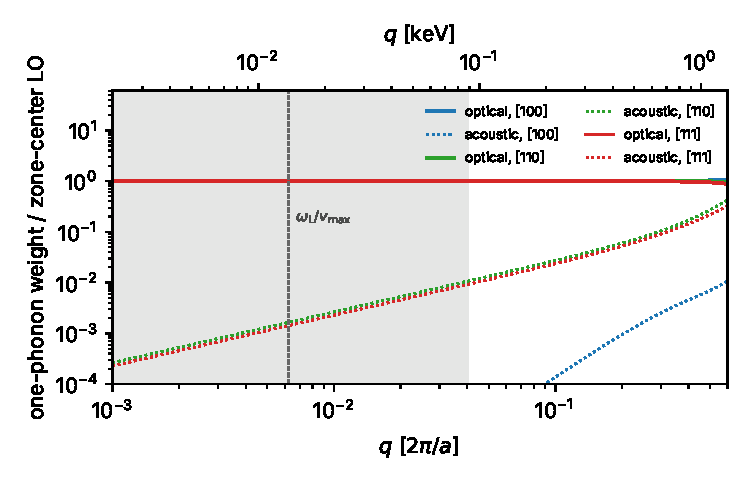
\includegraphics[width=\linewidth]{figures/ch11/limit11_2a.pdf}
\captionof{figure}{One-phonon weight of GaAs in \cref{eq:11.2-SZZ}, $\sum_\nu|\sum_\kappa\ee^{\ii\vect{q}\cdot\vect{\tau}_\kappa}\vect{e}^*_{\kappa\nu}\cdot Z^*_\kappa\cdot\hat{\vect{q}}/\sqrt{M_\kappa}|^2/2\omega_\nu$, divided by its zone-center value $Z^{*2}/2\mu_{\mathrm{red}}\omega_{\mathrm{L}}$, against $q$ along $[100]$, $[110]$ and $[111]$. Solid: the three optical branches; dotted: the three acoustic branches. Phonons at the actual $\vect{q}$ from the PBE force constants of \cref{fig:5-gaas}; Born charges held at their zone-center value. The ratios do not depend on $Z^*$ or $\varepsilon_\infty$. Gray: $q < 0.04 \times 2\pi/a = \SI{88}{eV}$, where the optical weight is within $10^{-4}$ of the formula and the acoustic weight is at most about \SI{1}{\percent}. Dashed line: $q = \omega_{\mathrm{L}}/v_{\mathrm{max}}$, the smallest momentum transfer that reaches the longitudinal phonon.}\label{fig:11-limit-2a}
\par}
\smallskip
At $q$ comparable with $2\pi/a$ the Born charge no longer describes the charge that moves with a nucleus, and the acoustic branches acquire a piezoelectric charge that the Born charges fix only in part.
\end{limitbox}

The optical weight stays within $10^{-4}$ of its zone-center value up to \SI{88}{eV} and within \SI{0.4}{\percent} up to \SI{450}{eV}, where the longitudinal branch has dispersed by \SI{0.3}{meV}. The acoustic branches are the leading correction, and they grow linearly in $q$: their weight reaches \SI{1}{\percent} of the optical one at \SI{90}{eV} along $[111]$ and \SI{5}{\percent} at \SI{450}{eV}, while along $[100]$ it vanishes by symmetry. This is the piezoelectric charge of \cref{sec:6.2}. With rigid Born charges an acoustic wave polarizes the cell only through the relative displacement of the sublattices that its strain induces; the dynamical quadrupoles of the displaced atoms, the next term beyond the Born charge in the expansion of the charge that moves with an atom in powers of $q$, add a contribution of the same order (\cref{app:E.5}), which the limit check does not include. The dotted curves are an estimate of the size of the correction.

The same order-$qa$ structure of the longitudinal mode sets the whole nucleon vertex of \cref{we:8-nucleon}, which vanishes as $q \to 0$; the charge vertex, finite at $q = 0$, is insensitive to it.

\subsection{The polar single-phonon rate}\label{sec:11.2-rate}

The dark matter enters through one potential. A dark photon couples to $-\tilde V n_Z$, with the same $\tilde V$ on electrons and nuclei, and we normalize it as for electron scattering, $|\tilde V|^2 = \pi\sigmae\FDM^2/\mu_{\chi e}^2$ (\cref{eq:1.4-Vsq}), with $\FDM = (q_0/q)^2$ for a light dark photon. We average the structure factor over the directions of $\vect{q}$, so that the halo enters through $\eta(\vmin)$ (\cref{eq:A.8-eta}); the direction dependence that a crystal keeps is the subject of \cref{sec:11.7}. With $S_{ZZ} = (2q^2/e^2)\bar L$ at $T = 0$, the rate \cref{eq:A.8-rateiso} becomes, for the light mediator,
\begin{keyresult}[Polar single-phonon rate]
\begin{equation}
  \mathcal{R} = \frac{\rho_\chi\,\sigmae\,q_0^4}{2\pi\,\mchi\,\mu_{\chi e}^2\,e^2\,\rho_T}\int_{\mathrm{band}}\dd\omega\;\bar L(\omega)\,K_\eta(\omega,\mchi) ,
  \qquad
  K_\eta(\omega,\mchi) = \int\frac{\dd q}{q}\;\eta\bigl(\vmin(q,\omega)\bigr) ,
  \label{eq:11.2-rate}
\end{equation}
with $\bar L$ the loss function at small $q$, averaged over directions, and the integral over the phonon band.
\end{keyresult}
\noindent All powers of $q$ cancel but one. A light mediator weights every logarithmic interval of momentum transfer equally, and the phonon fixes the energy deposited. The rate is then the loss function summed over the band, each line weighted by a kinematic factor that depends only on its energy and the dark-matter mass. Since $\vmin(q,\omega) \ge (2\omega/\mchi)^{1/2}$ at every $q$, the factor vanishes below the mass at which the fastest particle can deposit $\omega$, $2\omega/v_{\mathrm{max}}^2$ (\cref{eq:1.3-mmin}), which is \SI{10.35}{keV} for the longitudinal phonon of GaAs. For a single speed $v$, $\eta = \Theta(v - \vmin)/v$ and $K_\eta = \ln(q_+/q_-)/v$, with $q_\pm = \mchi v[1 \pm (1 - 2\omega/\mchi v^2)^{1/2}]$ the ends of the kinematic window.

For a heavy mediator, $\FDM = 1$, the same steps replace $K_\eta$ by $q_0^{-4}\int\dd q\,q^3\eta$, and the rate is weighted toward the largest momentum transfer, $2\mchi v_{\mathrm{max}}$. It leaves the region of \cref{fig:11-limit-2a}, where the acoustic share stays below a few percent, at about $0.2\times2\pi/a$, or $\mchi \approx \SI{83}{keV}$ in GaAs. The optical phonons alone keep the one-branch form to about \SI{0.1}{\percent} at \SI{99}{keV}; the vertex fails first.

\begin{figure}[tbp]
  \centering
  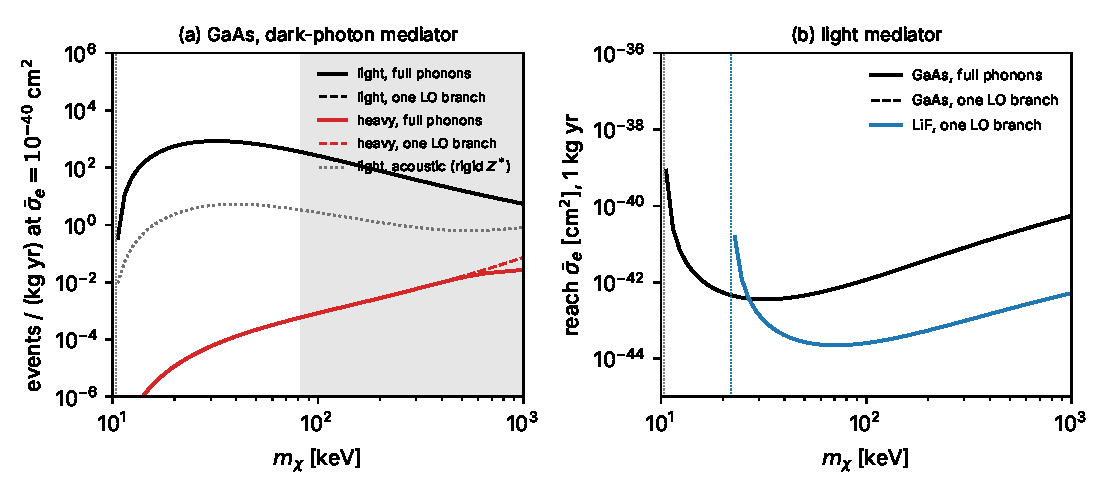
\includegraphics[width=\linewidth]{figures/ch11/fig11_2.pdf}
  \caption{Single-phonon scattering of dark matter through a dark photon in polar crystals, for the standard halo of \cref{sec:1.2} at $T = 0$. (a) Rate of GaAs per kilogram and year at $\sigmae = \SI{e-40}{cm^2}$, light ($\FDM = (q_0/q)^2$) and heavy ($\FDM = 1$) mediator. Solid: \cref{eq:11.2-SZZ} with the three optical branches of the PBE phonons of \cref{fig:5-gaas}, at the actual $\vect{q}$ (Umklapp included), averaged over 146 directions, in \cref{eq:A.8-rateiso}. Dashed: one longitudinal branch at the zone center, \cref{eq:11.2-onebranch} in \cref{eq:11.2-rate}. Both use $Z^* = 2.11$, the measured $\varepsilon_\infty = 10.88$, $\omega_{\mathrm{L}} = \SI{36.34}{meV}$ (DFPT) and $\rho_T = \SI{5.361}{g.cm^{-3}}$. Dotted: the acoustic branches with the same rigid Born charges and a \SI{1}{meV} threshold, an estimate of the piezoelectric correction (\cref{fig:11-limit-2a}). Gray: $2\mchi v_{\mathrm{max}} > 0.2\times2\pi/a$, where the Born-charge vertex is no longer reliable for the heavy mediator. (b) Light-mediator reach, three events in one kilogram-year without background: GaAs as in (a), and LiF with one longitudinal branch and the computed $Z^* = 1.05$, $\varepsilon_\infty = 2.02$ and $\omega_{\mathrm{L}} = \SI{77.2}{meV}$ of Ref.~\cite[Table~I]{griffin2020multichannel}. Vertical lines: the edges $2\omega_{\mathrm{L}}/v_{\mathrm{max}}^2 = 10.35$ and \SI{21.98}{keV}.}
  \label{fig:11-polar}
\end{figure}

\Cref{fig:11-polar}a shows the result for GaAs. The light-mediator rate rises from the edge to about 840 events per kilogram and year near \SI{29}{keV} for $\sigmae = \SI{e-40}{cm^2}$, and falls at larger masses as $\mu_{\chi e}^{-2}\mchi^{-1}$, with a logarithmic rise of $K_\eta$ on top. The full calculation agrees with the one-branch form to $3\times10^{-4}$ below \SI{300}{keV}; at \SI{1}{MeV} it is \SI{4}{\percent} lower, because part of the logarithmic integral then comes from momentum transfers beyond the zone. The acoustic branches, with rigid Born charges and a \SI{1}{meV} threshold, add at most \SI{3}{\percent}, near the edge, and about \SI{1}{\percent} at \SI{100}{keV}.

\subsection{The band integral}\label{sec:11.2-band}

GaAs has one polar branch, and the loss function has one line. By \cref{eq:5.5-eps}, $1/\varepsilon = \varepsilon_\infty^{-1}(\omega_{\mathrm{T}}^2 - \omega^2)/(\omega_{\mathrm{L}}^2 - \omega^2)$, whose pole at $\omega_{\mathrm{L}}$ leads to $L = (\pi\omega_{\mathrm{L}}/2)\varepsilon_\infty^{-1}(1 - \omega_{\mathrm{T}}^2/\omega_{\mathrm{L}}^2)\,\delta(\omega - \omega_{\mathrm{L}})$. By the Lyddane--Sachs--Teller relation the bracket is $1 - \varepsilon_\infty/\varepsilon_0$, and
\begin{equation}
  S_{ZZ}(\vect{q},\omega) = \frac{\pi q^2\omega_{\mathrm{L}}}{e^2}\Bigl(\frac{1}{\varepsilon_\infty} - \frac{1}{\varepsilon_0}\Bigr)\,\delta(\omega - \omega_{\mathrm{L}})
  = \frac{\pi q^2Z^{*2}}{\Omega\,\mu_{\mathrm{red}}\,\varepsilon_\infty^2\,\omega_{\mathrm{L}}}\,\delta(\omega - \omega_{\mathrm{L}}) .
  \label{eq:11.2-onebranch}
\end{equation}
The second form is \cref{eq:11.2-SZZ} with the longitudinal eigenvector of \cref{app:D.14}, $\vect{e}_1 = (M_2/M_{\mathrm{cell}})^{1/2}\hat{\vect{q}}$ and $\vect{e}_2 = -(M_1/M_{\mathrm{cell}})^{1/2}\hat{\vect{q}}$, for which $\sum_\kappa\vect{e}_\kappa\cdot Z^*_\kappa\cdot\vect{q}/\sqrt{M_\kappa} = Z^*q/\sqrt{\mu_{\mathrm{red}}}$; the two forms are equal by \cref{eq:5.5-LOTO,eq:5.5-LST}.

With several polar branches, how is the weight of $L$ shared among them? A sum rule answers part of the question exactly. The inverse-moment relation \cref{eq:4.4-inverse}, a consequence of causality alone, reads $(2/\pi)\int\dd\omega\,L/\omega = 1 - 1/\varepsilon_0$ for the total dielectric function and $1 - 1/\varepsilon_\infty$ with the nuclei clamped. Since the gap separates the two bands, the difference belongs to the phonons:
\begin{equation}
  \frac{2}{\pi}\int_{\mathrm{band}}\dd\omega\;\frac{L(\omega)}{\omega} = \frac{1}{\varepsilon_\infty} - \frac{1}{\varepsilon_0} .
  \label{eq:11.2-kk}
\end{equation}
At small $q$ the band is a set of lines, $L = \sum_\nu(\pi\omega_{\mathrm{L}\nu}/2)\,w^{\mathrm{pol}}_\nu\,\delta(\omega - \omega_{\mathrm{L}\nu})$, with the weights $w^{\mathrm{pol}}_\nu = e^2(\vect{p}\cdot\vect{e}_\nu)^2/(\Omega\varepsilon_\infty^2\omega_{\mathrm{L}\nu}^2)$ read off from the line formula above, and \cref{eq:11.2-kk} says that $\sum_\nu w^{\mathrm{pol}}_\nu = 1/\varepsilon_\infty - 1/\varepsilon_0$. The ionic part of the inverse static screening is shared out among the longitudinal branches. The rate needs the zeroth moment instead, the \emph{band integral}
\begin{equation}
  \begin{gathered}
  \mathcal{I}_{\mathrm{pol}} = \int_{\mathrm{band}}\dd\omega\;L(\omega) = \frac{\pi}{2}\sum_\nu\omega_{\mathrm{L}\nu}\,w^{\mathrm{pol}}_\nu , \\
  \frac{\pi}{2}\Bigl(\frac{1}{\varepsilon_\infty} - \frac{1}{\varepsilon_0}\Bigr)\omega_{\mathrm{L,min}} \le \mathcal{I}_{\mathrm{pol}} \le \frac{\pi}{2}\Bigl(\frac{1}{\varepsilon_\infty} - \frac{1}{\varepsilon_0}\Bigr)\omega_{\mathrm{T,max}}\Bigl(\frac{\varepsilon_0}{\varepsilon_\infty}\Bigr)^{1/2} ,
  \end{gathered}
  \label{eq:11.2-Ipol}
\end{equation}
bracketed by the sum rule. The upper end uses $\omega_{\mathrm{L,max}} \le \omega_{\mathrm{T,max}}(\varepsilon_0/\varepsilon_\infty)^{1/2}$, which holds because every ratio $\omega_{\mathrm{L}\nu}/\omega_{\mathrm{T}\nu}$ exceeds one and their squares multiply to $\varepsilon_0/\varepsilon_\infty$ (\cref{eq:D.14-LSTgen}). It needs only the transverse frequencies and the two dielectric constants.

In a crystal of lower symmetry these statements hold along each principal axis separately. Along a principal axis the lossless $\varepsilon$ of \cref{eq:11.2-eps} rises monotonically between consecutive poles, so that each transverse pole is followed by one longitudinal zero, $\omega_{\mathrm{T}1} < \omega_{\mathrm{L}1} < \omega_{\mathrm{T}2} < \dots$ (\cref{eq:D.14-LSTgen}), and $\varepsilon = \varepsilon_\infty\prod_\nu(\omega_{\mathrm{L}\nu}^2 - \omega^2)/(\omega_{\mathrm{T}\nu}^2 - \omega^2)$. The weights are then the residues of $-1/\varepsilon$ at its zeros, and the $\varepsilon_0$ and $\varepsilon_\infty$ of the sum rule must belong to the same axis and the same model. For a direction off the principal axes the zeros of $\hat{\vect{q}}\cdot\varepsilon\cdot\hat{\vect{q}}$ move with the direction, and the bracket applies axis by axis.

For a diatomic crystal, \cref{eq:11.2-onebranch} gives $\mathcal{I}_{\mathrm{pol}} = (\pi/2)e^2Z^{*2}/(\Omega\mu_{\mathrm{red}}\varepsilon_\infty^2\omega_{\mathrm{L}})$, and per unit mass, with $\rho_T = M_{\mathrm{cell}}/\Omega$,
\begin{equation}
  \frac{\mathcal{I}_{\mathrm{pol}}}{\rho_T} = \frac{\pi}{2}\,\frac{e^2Z^{*2}}{M_{\mathrm{cell}}\,\mu_{\mathrm{red}}\,\varepsilon_\infty^2\,\omega_{\mathrm{L}}} ,
  \label{eq:11.2-diatomic}
\end{equation}
in which the cell volume has dropped out. In general \cref{eq:11.2-rate} is a sum over branches, $\sum_\nu(\pi\omega_{\mathrm{L}\nu}/2)(w^{\mathrm{pol}}_\nu/\rho_T)K_\eta(\omega_{\mathrm{L}\nu},\mchi)$. When $K_\eta$ changes little across the band, it is $\mathcal{I}_{\mathrm{pol}}/\rho_T$ times $K_\eta$ at the weighted mean frequency $\bar\omega_{\mathrm{pol}} = \sum_\nu\omega_{\mathrm{L}\nu}w^{\mathrm{pol}}_\nu/\sum_\nu w^{\mathrm{pol}}_\nu$, and the material enters through $\mathcal{I}_{\mathrm{pol}}/\rho_T$ alone. Sapphire, with four polar branches on its ordinary axis, tests this reading.

\begin{limitbox}[Polar band integral][lim:11.2b]
For one polar branch the light-mediator rate is \cref{eq:11.2-rate} with the line \cref{eq:11.2-onebranch}~\cite[Eqs.~(21), (22), (24)]{griffin2018directional}; with several branches the light-mediator rate per unit mass is proportional to $\mathcal{I}_{\mathrm{pol}}/\rho_T$.
\par\smallskip
{\centering
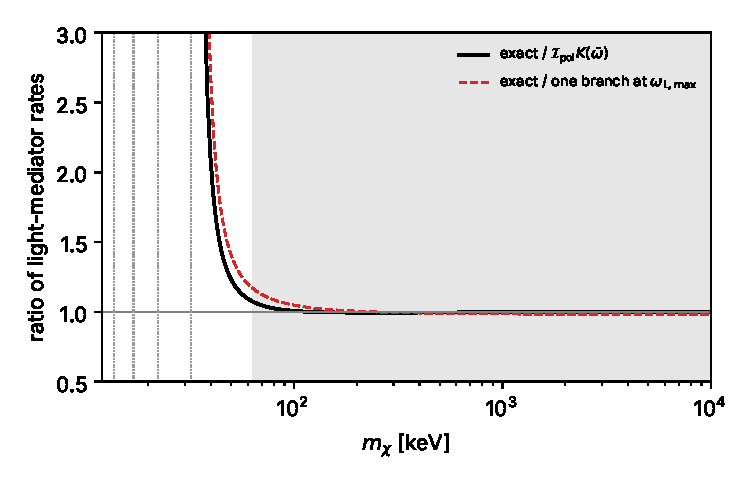
\includegraphics[width=\linewidth]{figures/ch11/limit11_2b.pdf}
\captionof{figure}{Light-mediator rate of the ordinary axis of sapphire, the exact sum over its four longitudinal branches, divided by the band-integral form $\mathcal{I}_{\mathrm{pol}}K_\eta(\bar\omega_{\mathrm{pol}},\mchi)$ (solid) and by the one-branch form with the highest longitudinal frequency and the same $1/\varepsilon_\infty - 1/\varepsilon_0$ (dashed), against $\mchi$. Lossless factorized $\varepsilon$ from the measured frequencies of Ref.~\cite[Table~II]{griffin2018directional} (ordinary ray: longitudinal 112.4, 78.0, 59.7, \SI{48.1}{meV}; transverse 78.6, 70.5, 54.4, \SI{47.7}{meV}) and $\varepsilon_\infty = 3.2$~\cite[Table~I]{griffin2018directional}; weights from the residues of $-1/\varepsilon$, $\bar\omega_{\mathrm{pol}} = \SI{109.9}{meV}$; standard halo of \cref{sec:1.2}. Dotted lines: the four edges $2\omega_{\mathrm{L}\nu}/v_{\mathrm{max}}^2$, from 13.7 to \SI{32.0}{keV}. Gray: $\mchi$ above twice the highest edge, \SI{64}{keV}, where the band-integral form is within \SI{7}{\percent}.}\label{fig:11-limit-2b}
\par}
\smallskip
Within about twice the highest edge the branches open one by one, the lowest first, and the rate follows the individual longitudinal frequencies rather than their weighted sum.
\end{limitbox}

On the ordinary axis of sapphire one branch takes almost all the weight. The longitudinal phonon at \SI{112.4}{meV} carries \SI{95.2}{\percent} of $1/\varepsilon_\infty - 1/\varepsilon_0 = 0.210$. It is a collective mode: the macroscopic field of all the dipoles together pushes it up to \SI{112.4}{meV}, and like a plasmon it collects nearly all of the loss weight. Its band integral is $\mathcal{I}_{\mathrm{pol}} = \SI{36.3}{meV}$, about \SI{70}{\percent} of the way up the bracket \cref{eq:11.2-Ipol}, $[15.9, 45.4]$\,meV. With the highest longitudinal frequency itself, \SI{112.4}{meV}, in place of its bound $\omega_{\mathrm{T,max}}(\varepsilon_0/\varepsilon_\infty)^{1/2}$, the upper end tightens to \SI{37.1}{meV}. With $\rho_T = \SI{3.98}{g.cm^{-3}}$~\cite[Table~I]{griffin2018directional}, $\mathcal{I}_{\mathrm{pol}}/\rho_T = \SI{9.12}{meV.cm^3.g^{-1}}$. Above \SI{64}{keV} the band-integral form is good to \SI{7}{\percent}. At \SI{40}{keV}, however, the true rate is 2.1 times the band-integral form, because the branches between 48 and \SI{78}{meV} are already well open while the dominant one has barely opened. Damping adds a correction of order $\gamma_{\mathrm{L}}/\omega_{\mathrm{L}}$, the width of the line over its frequency. For the dominant phonon of sapphire, $\gamma_{\mathrm{L}} = \SI{16}{cm^{-1}}$ at \SI{77}{K}~\cite[Table~II]{griffin2018directional}, or \SI{1.8}{\percent}; the Lorentzian line adds weight in its tails.

\subsection{The Born charge from the splitting}\label{sec:11.2-split}

For a diatomic crystal the rate needs one combination of material numbers, $Z^*/\varepsilon_\infty$, the screened dipole per unit displacement. Solving \cref{eq:5.5-LOTO} for it,
\begin{equation}
  \frac{Z^*}{\varepsilon_\infty} = \Bigl[\frac{\Omega\,\mu_{\mathrm{red}}\,(\omega_{\mathrm{L}}^2 - \omega_{\mathrm{T}}^2)}{e^2\,\varepsilon_\infty}\Bigr]^{1/2} ,
  \label{eq:11.2-Zeps}
\end{equation}
which needs two phonon frequencies, the cell, the masses and $\varepsilon_\infty$, but not the static constant. For GaAs, \cref{we:5-lst} has already extracted $Z^* = 2.11$ from the measured splitting, and by \cref{eq:11.2-Zeps} $Z^*/\varepsilon_\infty = 0.194$. The error budget follows from the logarithmic derivative,
\begin{equation*}
  \frac{\delta(Z^*/\varepsilon_\infty)}{Z^*/\varepsilon_\infty} = -\frac12\frac{\delta\varepsilon_\infty}{\varepsilon_\infty} + \frac{\omega_{\mathrm{L}}\,\delta\omega_{\mathrm{L}} - \omega_{\mathrm{T}}\,\delta\omega_{\mathrm{T}}}{\omega_{\mathrm{L}}^2 - \omega_{\mathrm{T}}^2} .
\end{equation*}
A common calibration error of the two frequencies cancels to first order. Independent errors are amplified by $\omega^2/(\omega_{\mathrm{L}}^2 - \omega_{\mathrm{T}}^2) \approx 6.9$, so that \SI{0.1}{\percent} on each frequency costs \SI{0.9}{\percent}, and together with \SI{1}{\percent} on $\varepsilon_\infty$ the result is good to \SI{1.0}{\percent}. The dielectric constant should be the one at the temperature of the detector, since it changes at the percent level between room temperature and liquid-helium temperature~\cite{griffin2018directional}.

\subsection{Rate and reach of polar targets}\label{sec:11.2-targets}

\begin{workedexample}{The band integral of GaAs and LiF}\label{we:11-ipol}
GaAs has one polar branch, and \cref{eq:11.2-Ipol} has one term. We take the measured numbers of \cref{we:5-lst} and its cell, $a = \SI{5.638}{\angstrom}$, the static-lattice constant of \cref{tab:E-functionals}, the measured value with the thermal and zero-point expansion removed, which is also the cell of the computed phonons; then $\rho_T = M_{\mathrm{cell}}/\Omega = \SI{144.645}{u}/\SI{44.80}{\angstrom^3} = \SI{5.361}{g.cm^{-3}}$.

\emph{Through the dielectric constants.} $1/\varepsilon_\infty - 1/\varepsilon_0 = 1/10.88 - 1/12.9 = 0.01439$, so that $\mathcal{I}_{\mathrm{pol}} = (\pi/2)(\SI{36.35}{meV})(0.01439) = \SI{0.822}{meV}$ and $\mathcal{I}_{\mathrm{pol}}/\rho_T = \SI{0.153}{meV.cm^3.g^{-1}}$.

\emph{Through the splitting.} By the Lyddane--Sachs--Teller relation $1/\varepsilon_\infty - 1/\varepsilon_0 = (1 - \omega_{\mathrm{T}}^2/\omega_{\mathrm{L}}^2)/\varepsilon_\infty$, and $\mathcal{I}_{\mathrm{pol}} = (\pi/2)(\omega_{\mathrm{L}}^2 - \omega_{\mathrm{T}}^2)/(\varepsilon_\infty\omega_{\mathrm{L}}) = \SI{0.759}{meV}$, or $\SI{0.1415}{meV.cm^3.g^{-1}}$ per unit mass. The two routes differ by \SI{8}{\percent}: the \SI{1.4}{\percent} residual of the inputs, amplified by $\partial\ln\mathcal{I}_{\mathrm{pol}}/\partial\ln\varepsilon_0 = \varepsilon_\infty/(\varepsilon_0 - \varepsilon_\infty) = 5.4$.

\emph{From a table of computed values.} The target table of Griffin and collaborators lists $Z^* = 2.27$, $\varepsilon_\infty = 10.9$ and optical energies from 31.8 to \SI{34.9}{meV} for GaAs~\cite[Table~I]{griffin2020multichannel}. In \cref{eq:11.2-diatomic}, with $M_{\mathrm{cell}} = \SI{144.645}{u}$ and $\mu_{\mathrm{red}} = \SI{36.11}{u}$, they give \SI{0.170}{meV.cm^3.g^{-1}}, \SI{20}{\percent} above the splitting route, mostly because their Born charge is \SI{8}{\percent} above the measured one.

\emph{LiF.} The same table gives $Z^* = 1.05$, $\varepsilon_\infty = 2.02$ and optical energies from 33.5 to \SI{77.2}{meV}. With $M_{\mathrm{cell}} = \SI{25.94}{u}$ and $\mu_{\mathrm{red}} = \SI{5.084}{u}$, \cref{eq:11.2-diatomic} yields $\mathcal{I}_{\mathrm{pol}}/\rho_T = \SI{19.0}{meV.cm^3.g^{-1}}$, 112 times the GaAs value of the same table. The factors are: the weaker electronic screening gains $(10.9/2.02)^2 = 29$ and the lighter ions $M_{\mathrm{cell}}\mu_{\mathrm{red}}$ a factor of 40, while the smaller Born charge gives back $(1.05/2.27)^2 = 0.21$ and the higher frequency $34.9/77.2 = 0.45$.

\emph{Edges.} The lightest masses that reach the longitudinal phonon are $2\omega_{\mathrm{L}}/v_{\mathrm{max}}^2 = \SI{10.35}{keV}$ for GaAs and \SI{21.98}{keV} for LiF.
\end{workedexample}

At large mass the kinematic weights of the two crystals approach each other: at \SI{1}{MeV}, $K_\eta$ of LiF is 0.77 times that of GaAs. LiF then leads by a factor of 103, the ratio 134 of its band integral to the splitting value of GaAs, times 0.77. Toward lower masses the ratio falls, to 46 at \SI{100}{keV}, 17 at \SI{50}{keV} and 2.6 at \SI{30}{keV}; at \SI{25}{keV} GaAs is ahead, and below \SI{22}{keV} the rate of LiF vanishes. \Cref{fig:11-polar}b shows the consequence for the reach: the two curves cross at \SI{26.7}{keV}, and below it only GaAs has reach.

The order of polar targets by rate is reversed in their reach, and the reversal is general. Write the diatomic band integral with the splitting, $\mathcal{I}_{\mathrm{pol}}/\rho_T = (\pi/2)(\omega_{\mathrm{L}}/\varepsilon_\infty\rho_T)(1 - \omega_{\mathrm{T}}^2/\omega_{\mathrm{L}}^2)$. At a given screening, density and ratio of the two frequencies, the band integral is proportional to $\omega_{\mathrm{L}}$, and so is the edge $2\omega_{\mathrm{L}}/v_{\mathrm{max}}^2$. The light ions that make $\mathcal{I}_{\mathrm{pol}}$ large are the ones that make the phonon hard, through the reduced mass in $\omega_{\mathrm{T}}^2 = C_0/\mu_{\mathrm{red}}$ and in the splitting \cref{eq:5.5-LOTO}. A crystal of heavy, soft ions, such as CsI with optical modes between 6.9 and \SI{10.0}{meV}~\cite[Table~I]{griffin2020multichannel}, reaches down to \SI{2.85}{keV}, but with a far smaller rate above that. The best polar crystal depends on the mass window, and \cref{sec:17.5} poses it as a figure of merit.
